% Practice Test 19 — Texas Edition
% Questions: 30 (23 MC + 7 SA)
% Generated by scripts/generate_practice_tests.py

\begin{practiceQuestion}{1-3-q01}{mc}
\begin{questionText}
What is the constant of proportionality ($k$) for the table below?

\begin{center}
\begin{tabular}{|c|c|}
\hline $x$ & $y$ \\ \hline $3$ & $12$ \\ $5$ & $20$ \\ $8$ & $32$ \\ \hline
\end{tabular}
\end{center}
\end{questionText}
\choiceA{$3$}
\choiceB{$4$}
\choiceC{$8$}
\choiceD{$12$}
\correctAnswer{B}
\explanation{$k = \frac{y}{x} = \frac{12}{3} = 4$. Check: $\frac{20}{5} = 4$ and $\frac{32}{8} = 4$.}
\end{practiceQuestion}

\begin{practiceQuestion}{1-6-q25}{sa}
\begin{questionText}
A truck delivers $540$ packages in $3$ trips. How many trips are needed to deliver $1{,}620$ packages?
\end{questionText}
\correctAnswer{$9$ trips}
\explanation{Per trip: $540 \div 3 = 180$ packages. Trips needed: $1{,}620 \div 180 = 9$.}
\end{practiceQuestion}

\begin{practiceQuestion}{2-1-q16}{mc}
\begin{questionText}
$9$ is $12\%$ of what number?
\end{questionText}
\choiceA{$1.08$}
\choiceB{$36$}
\choiceC{$72$}
\choiceD{$75$}
\correctAnswer{D}
\explanation{Divide the part by the percent: $9 \div 0.12 = 75$.}
\end{practiceQuestion}

\begin{practiceQuestion}{2-3-q22}{sa}
\begin{questionText}
A pond had $400$ fish last year and $340$ this year. What is the percent decrease?


\numberLine[10]{340}{410}
\end{questionText}
\correctAnswer{$15\%$}
\explanation{Change: $400 - 340 = 60$. Percent decrease: $60 \div 400 = 0.15 = 15\%$.}
\end{practiceQuestion}

\begin{practiceQuestion}{2-6-q01}{mc}
\begin{questionText}
Find the simple interest: $P = \$500$, $r = 6\%$, $t = 3$ years.
\end{questionText}
\choiceA{$\$30$}
\choiceB{$\$60$}
\choiceC{$\$90$}
\choiceD{$\$150$}
\correctAnswer{C}
\explanation{$I = Prt = 500 \times 0.06 \times 3 = \$90$.}
\end{practiceQuestion}

\begin{practiceQuestion}{2-8-q03}{mc}
\begin{questionText}
A credit union is most similar to which of the following?
\end{questionText}
\choiceA{A department store}
\choiceB{A bank}
\choiceC{A stock market}
\choiceD{A government office}
\correctAnswer{B}
\explanation{A credit union works like a bank (savings, checking, loans) but is owned by its members and often has lower fees.}
\end{practiceQuestion}

\begin{practiceQuestion}{2-9-q18}{mc}
\begin{questionText}
Which formula correctly represents the relationship between income, expenses, and savings?
\end{questionText}
\choiceA{Income $=$ Savings $+$ Expenses}
\choiceB{Savings $=$ Expenses $-$ Income}
\choiceC{Income $=$ Expenses $-$ Savings}
\choiceD{Expenses $=$ Income $+$ Savings}
\correctAnswer{A}
\explanation{Income $-$ Expenses $=$ Savings, which can be rearranged to Income $=$ Savings $+$ Expenses.}
\end{practiceQuestion}

\begin{practiceQuestion}{2-10-q21}{sa}
\begin{questionText}
$\$900$ at $10\%$ compounded yearly for $3$ years. What is the total amount?
\end{questionText}
\correctAnswer{$\$1{,}197.90$}
\explanation{Year 1: $900 \times 1.10 = 990$. Year 2: $990 \times 1.10 = 1{,}089$. Year 3: $1{,}089 \times 1.10 = \$1{,}197.90$.}
\end{practiceQuestion}

\begin{practiceQuestion}{4-1-q11}{mc}
\begin{questionText}
Which expression represents ``the product of $7$ and a number $p$, decreased by $12$''?
\end{questionText}
\choiceA{$7(p - 12)$}
\choiceB{$12 - 7p$}
\choiceC{$7p - 12$}
\choiceD{$7 + p - 12$}
\correctAnswer{C}
\explanation{``The product of $7$ and $p$'' is $7p$. ``Decreased by $12$'' means subtract $12$: $7p - 12$.}
\end{practiceQuestion}

\begin{practiceQuestion}{4-2-q02}{mc}
\begin{questionText}
Simplify $7x + 3x$.
\end{questionText}
\choiceA{$10x$}
\choiceB{$21x$}
\choiceC{$10x^2$}
\choiceD{$73x$}
\correctAnswer{A}
\explanation{$7x$ and $3x$ are like terms. Add the coefficients: $7 + 3 = 10$. Result: $10x$.}
\end{practiceQuestion}

\begin{practiceQuestion}{5-3-q12}{mc}
\begin{questionText}
Solve $7(x - 2) = 0$.
\end{questionText}
\choiceA{$x = 0$}
\choiceB{$x = -2$}
\choiceC{$x = 2$}
\choiceD{$x = 7$}
\correctAnswer{C}
\explanation{Divide by $7$: $x - 2 = 0$. Add $2$: $x = 2$. Check: $7(2 - 2) = 7(0) = 0$ \checkmark.}
\end{practiceQuestion}

\begin{practiceQuestion}{5-4-q21}{sa}
\begin{questionText}
Solve $\dfrac{x}{2} + \dfrac{x}{4} = 9$.
\end{questionText}
\correctAnswer{$x = 12$}
\explanation{Multiply every term by $4$: $2x + x = 36$. Combine: $3x = 36$. Divide by $3$: $x = 12$. Check: $\frac{12}{2} + \frac{12}{4} = 6 + 3 = 9$ \checkmark.}
\end{practiceQuestion}

\begin{practiceQuestion}{5-5-q27}{gmc}
\begin{questionText}
Look at the number line. Which inequality has this solution?

\begin{center}
\begin{tikzpicture}[scale=0.7]
  \draw[thick,->] (-6,0) -- (4,0);
  \foreach \x in {-5,...,3} \draw (\x,0.15) -- (\x,-0.15) node[below] {$\x$};
  \draw[thick,funOrange,<-] (-6,0) -- (-2,0);
  \fill[funOrange] (-2,0) circle (4pt);
\end{tikzpicture}
\end{center}
\end{questionText}
\choiceA{$3x + 1 > -5$}
\choiceB{$-4x \geq 8$}
\choiceC{$2x - 3 < -7$}
\choiceD{$x + 5 > 3$}
\correctAnswer{B}
\explanation{The graph shows $x \leq -2$ (closed circle, shading left). $-4x \geq 8$: divide by $-4$ and flip: $x \leq -2$ \checkmark.}
\end{practiceQuestion}

\begin{practiceQuestion}{5-6-q22}{sa}
\begin{questionText}
Solve $10 - 4x < 2$. Describe the graph.
\end{questionText}
\correctAnswer{$x > 2$; open circle at $2$, shade right}
\explanation{Subtract $10$: $-4x < -8$. Divide by $-4$ and flip: $x > 2$. Open circle at $2$, shade right.}
\end{practiceQuestion}

\begin{practiceQuestion}{6-2-q06}{mc}
\begin{questionText}
A map uses $1$ cm $= 20$ km. You redraw it at $1$ cm $= 10$ km. What happens to the drawing?
\end{questionText}
\choiceA{Every length is halved}
\choiceB{Every length stays the same}
\choiceC{Every length is doubled}
\choiceD{Every length is multiplied by $10$}
\correctAnswer{C}
\explanation{Scale ratio: $\frac{20}{10} = 2$. Every length on the new drawing is $2$ times the old one. The drawing gets bigger because each cm now represents fewer real km.}
\end{practiceQuestion}

\begin{practiceQuestion}{6-3-q28}{gmc}
\begin{questionText}
The four rectangles below all have the same perimeter of $16$ cm but different dimensions. What does this tell us?

\begin{center}
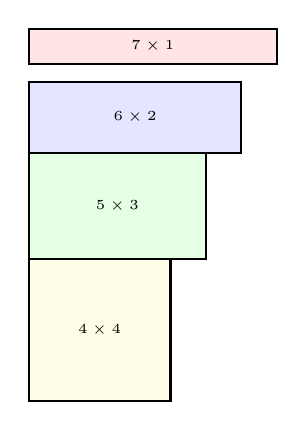
\begin{tikzpicture}[scale=0.45]
  \draw[thick,fill=red!10] (0,0) rectangle (7,1);
  \node at (3.5,0.5) {\tiny $7 \times 1$};
  \draw[thick,fill=blue!10] (0,-2.5) rectangle (6,-0.5);
  \node at (3,-1.5) {\tiny $6 \times 2$};
  \draw[thick,fill=green!10] (0,-5.5) rectangle (5,-2.5);
  \node at (2.5,-4) {\tiny $5 \times 3$};
  \draw[thick,fill=yellow!10] (0,-9.5) rectangle (4,-5.5);
  \node at (2,-7.5) {\tiny $4 \times 4$};
\end{tikzpicture}
\end{center}
\end{questionText}
\choiceA{A given perimeter determines exactly one rectangle}
\choiceB{A given perimeter allows more than one rectangle}
\choiceC{All rectangles with the same perimeter have the same area}
\choiceD{It is impossible for multiple rectangles to share a perimeter}
\correctAnswer{B}
\explanation{The four rectangles all have perimeter $16$ cm ($2(7+1) = 2(6+2) = 2(5+3) = 2(4+4) = 16$) but different shapes. A given perimeter allows many rectangles.}
\end{practiceQuestion}

\begin{practiceQuestion}{6-4-q14}{mc}
\begin{questionText}
Sides $5$, $12$, $13$. Is this a right triangle?
\end{questionText}
\choiceA{No, because $5 + 12 \neq 13$}
\choiceB{No, because the sides are not equal}
\choiceC{Yes, because $5^2 + 12^2 = 13^2$}
\choiceD{Yes, because $5 + 12 = 17 > 13$}
\correctAnswer{C}
\explanation{$5^2 + 12^2 = 25 + 144 = 169 = 13^2$. The Pythagorean theorem holds, so it is a right triangle.}
\end{practiceQuestion}

\begin{practiceQuestion}{6-5-q13}{mc}
\begin{questionText}
A hexagonal prism is sliced parallel to its base. What is the cross-section?
\end{questionText}
\choiceA{Rectangle}
\choiceB{Triangle}
\choiceC{Hexagon}
\choiceD{Circle}
\correctAnswer{C}
\explanation{Any cut parallel to the base of a prism gives a shape congruent to the base. A hexagonal prism has a hexagonal base, so the cross-section is a hexagon.}
\end{practiceQuestion}

\begin{practiceQuestion}{6-8-q14}{mc}
\begin{questionText}
Triangle $LMN \sim$ Triangle $XYZ$. $LM = 10$, $MN = 14$, $LN = 16$, $XY = 5$. Find $YZ$.
\end{questionText}
\choiceA{$7$}
\choiceB{$8$}
\choiceC{$9$}
\choiceD{$28$}
\correctAnswer{A}
\explanation{Scale factor: $\frac{5}{10} = 0.5$. $YZ = 14 \times 0.5 = 7$.}
\end{practiceQuestion}

\begin{practiceQuestion}{7-4-q09}{mc}
\begin{questionText}
A banner is shaped like a rectangle $18$ in by $6$ in with a triangle cut from one end. The triangle has a base of $6$ in and a height of $4$ in. What is the area of the banner?
\end{questionText}
\choiceA{$84$ in$^2$}
\choiceB{$96$ in$^2$}
\choiceC{$108$ in$^2$}
\choiceD{$120$ in$^2$}
\correctAnswer{B}
\explanation{Rectangle: $18 \times 6 = 108$ in$^2$. Triangle: $\frac{1}{2} \times 6 \times 4 = 12$ in$^2$. Banner: $108 - 12 = 96$ in$^2$.}
\end{practiceQuestion}

\begin{practiceQuestion}{7-5-q04}{mc}
\begin{questionText}
How many faces does a rectangular prism have?
\end{questionText}
\choiceA{$4$}
\choiceB{$5$}
\choiceC{$6$}
\choiceD{$8$}
\correctAnswer{C}
\explanation{A rectangular prism has $6$ faces: top, bottom, front, back, left, and right.}
\end{practiceQuestion}

\begin{practiceQuestion}{7-6-q09}{mc}
\begin{questionText}
What unit is used to measure volume?
\end{questionText}
\choiceA{Square units (cm$^2$)}
\choiceB{Cubic units (cm$^3$)}
\choiceC{Linear units (cm)}
\choiceD{Degrees}
\correctAnswer{B}
\explanation{Volume measures three-dimensional space and is measured in cubic units.}
\end{practiceQuestion}

\begin{practiceQuestion}{8-1-q27}{gmc}
\begin{questionText}
The diagram below shows four different sampling methods used to survey students at a school. Which method is most likely to produce an unbiased sample?

\begin{center}
\begin{tikzpicture}[scale=0.75]
  % Method A
  \node[draw,rounded corners,fill=funBlue!15,minimum width=3.5cm,minimum height=1.2cm,align=center] (A) at (0,3) {\textbf{Method A}\\Survey the football team};
  % Method B
  \node[draw,rounded corners,fill=funGreen!15,minimum width=3.5cm,minimum height=1.2cm,align=center] (B) at (6,3) {\textbf{Method B}\\Survey every 10th student\\on the school roster};
  % Method C
  \node[draw,rounded corners,fill=funOrange!15,minimum width=3.5cm,minimum height=1.2cm,align=center] (C) at (0,0) {\textbf{Method C}\\Post survey online and\\wait for responses};
  % Method D
  \node[draw,rounded corners,fill=funRed!15,minimum width=3.5cm,minimum height=1.2cm,align=center] (D) at (6,0) {\textbf{Method D}\\Survey students in\\one math class};
\end{tikzpicture}
\end{center}
\end{questionText}
\choiceA{Method A}
\choiceB{Method B}
\choiceC{Method C}
\choiceD{Method D}
\correctAnswer{B}
\explanation{Selecting every 10th student from the school roster is systematic and gives all students a chance, making it the least biased.}
\end{practiceQuestion}

\begin{practiceQuestion}{8-2-q22}{sa}
\begin{questionText}
A sample of $40$ students found that $10$ prefer vanilla ice cream. If the school has $800$ students, predict how many prefer vanilla.
\end{questionText}
\correctAnswer{$200$}
\explanation{$\frac{10}{40} = 25\%$. Then $25\%$ of $800 = 200$.}
\end{practiceQuestion}

\begin{practiceQuestion}{8-4-q03}{mc}
\begin{questionText}
Group A has a mean of $50$ and a MAD of $3$. Group B has a mean of $60$ and a MAD of $3$. The difference in means expressed in MADs is:
\end{questionText}
\choiceA{$\frac{10}{3} \approx 3.3$ MADs}
\choiceB{$10$ MADs}
\choiceC{$3$ MADs}
\choiceD{$30$ MADs}
\correctAnswer{A}
\explanation{Difference $= 60 - 50 = 10$. In MADs: $\frac{10}{3} \approx 3.3$.}
\end{practiceQuestion}

\begin{practiceQuestion}{8-5-q13}{mc}
\begin{questionText}
Data: $45, 48, 52, 55, 55, 58, 61, 63$. Which is the correct stem-and-leaf plot?
\end{questionText}
\choiceA{Stems: $4, 5, 6$; Row $4$: $5\;\;8$; Row $5$: $2\;\;5\;\;5\;\;8$; Row $6$: $1\;\;3$}
\choiceB{Stems: $4, 5, 6$; Row $4$: $5\;\;8$; Row $5$: $5\;\;5\;\;2\;\;8$; Row $6$: $3\;\;1$}
\choiceC{Stems: $45, 48, 52$; no leaves}
\choiceD{Stems: $4, 5$; Row $4$: $5\;\;8$; Row $5$: $2\;\;5\;\;5\;\;8\;\;1\;\;3$}
\correctAnswer{A}
\explanation{Stems are tens digits ($4, 5, 6$), leaves are ones digits listed in order. Only choice A has correct stems and ordered leaves.}
\end{practiceQuestion}

\begin{practiceQuestion}{8-6-q16}{mc}
\begin{questionText}
A student creates a circle graph with sectors of $100°$, $80°$, $60°$, and $100°$. Is this circle graph correct?
\end{questionText}
\choiceA{Yes — the sectors look reasonable}
\choiceB{No — the angles add to $340°$, not $360°$}
\choiceC{No — there are too many sectors}
\choiceD{Yes — all angles are less than $180°$}
\correctAnswer{B}
\explanation{$100 + 80 + 60 + 100 = 340°$, which is $20°$ short of $360°$. The graph is incorrect.}
\end{practiceQuestion}

\begin{practiceQuestion}{9-4-q07}{mc}
\begin{questionText}
A coin is weighted so that heads comes up $60\%$ of the time. What is the probability of tails?
\end{questionText}
\choiceA{$0.60$}
\choiceB{$0.50$}
\choiceC{$0.40$}
\choiceD{$0.30$}
\correctAnswer{C}
\explanation{$P(\text{tails}) = 1 - 0.60 = 0.40$. Since heads and tails have different probabilities, this is a non-uniform model.}
\end{practiceQuestion}

\begin{practiceQuestion}{9-6-q30}{gsa}
\begin{questionText}
Look at the tree diagram for flipping three coins. What is the probability of getting exactly $2$ tails? Write your answer as a fraction in simplest form.

\begin{center}
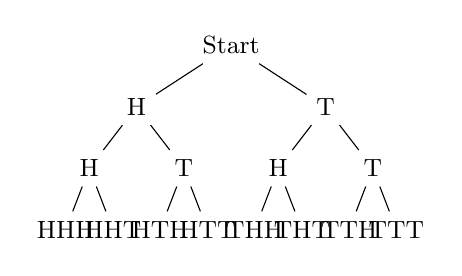
\begin{tikzpicture}[scale=0.6,
  level 1/.style={sibling distance=4cm, level distance=1.3cm},
  level 2/.style={sibling distance=2cm, level distance=1.3cm},
  level 3/.style={sibling distance=1cm, level distance=1.3cm}]
  \node {\small Start}
    child {node {\small H}
      child {node {\small H}
        child {node {\small HHH}}
        child {node {\small HHT}}
      }
      child {node {\small T}
        child {node {\small HTH}}
        child {node {\small HTT}}
      }
    }
    child {node {\small T}
      child {node {\small H}
        child {node {\small THH}}
        child {node {\small THT}}
      }
      child {node {\small T}
        child {node {\small TTH}}
        child {node {\small TTT}}
      }
    };
\end{tikzpicture}
\end{center}
\end{questionText}
\correctAnswer{$\frac{3}{8}$}
\explanation{Outcomes with exactly $2$ tails: HTT, THT, TTH — that is $3$ out of $8$. $P = \frac{3}{8}$.}
\end{practiceQuestion}

\begin{practiceQuestion}{9-7-q17}{mc}
\begin{questionText}
A student wants to simulate the probability that exactly $2$ out of $3$ students pass a test, where each student has a $50\%$ chance. Which model would work?
\end{questionText}
\choiceA{Roll one die: odd = pass, even = fail}
\choiceB{Flip $3$ coins: heads = pass, tails = fail; count exactly $2$ heads}
\choiceC{Draw $3$ marbles from a bag of $2$ red and $1$ blue}
\choiceD{Flip $1$ coin $3$ times and count all tails}
\correctAnswer{B}
\explanation{Each coin flip has a $50\%$ chance of heads (pass). Flipping $3$ coins and counting exactly $2$ heads simulates exactly $2$ passes.}
\end{practiceQuestion}
